\documentclass[12pt, twoside]{article}
\usepackage[letterpaper, margin=1in, headsep=0.5in]{geometry}
\usepackage[english]{babel}
\usepackage[utf8]{inputenc}
\usepackage{amsmath}
\usepackage{amsfonts}
\usepackage{amssymb}
\usepackage{tikz}
\usetikzlibrary{quotes, angles}
\usepackage{graphicx}
\usepackage{enumitem}
\usepackage{multicol}

\newif\ifmeta
\metatrue %print standards and topics tags

\title{Regents Geometry}
\author{Chris Huson}
\date{September 2020}

\usepackage{fancyhdr}
\pagestyle{fancy}
\fancyhf{}
\renewcommand{\headrulewidth}{0pt} % disable the underline of the header
\raggedbottom


\fancyhead[LE]{\thepage}
\fancyhead[RO]{\thepage \\ Name: \hspace{4cm} \,\\}
\fancyhead[L]{BECA / Dr. Huson / Geometry 05-Transformations\\* pset ID: 71}

\begin{document}

\subsubsection*{5-9bDN-Multi-step}
\begin{enumerate}
\item A translation maps triangle $PQR$ onto triangle $STU$. \vspace{0.5cm}
    \begin{multicols}{2}  
    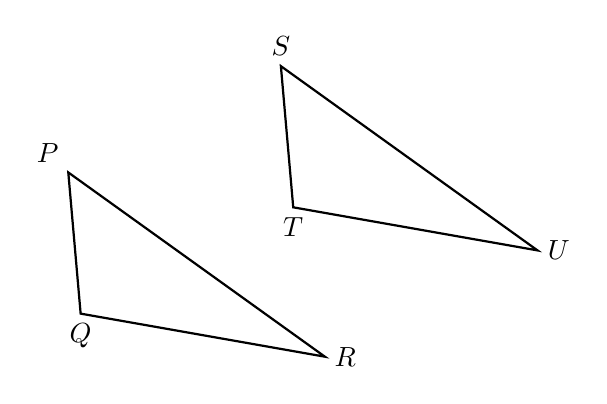
\begin{tikzpicture}[scale=0.9]
        \coordinate [label=above left:$P$](A) at (95:2);
        \coordinate [label=below:$Q$](B) at (0, 0);
        \coordinate [label=right:$R$](C) at (-10:3.5);
        \draw [thick] (A)--(B)--(C)--cycle;
  
        \draw [thick, xshift=3cm, yshift=1.5cm] (95:2) node[above]{$S$}--
        (0,0) node[below]{$T$}--
        (-10:3.5) node[right]{$U$}--cycle;
      \end{tikzpicture}\\
      Write each corresponding object.
      \begin{enumerate}
        \item $Q \rightarrow$ \rule{2cm}{0.15mm}
        \item $\angle QRP \cong$ \rule{2cm}{0.15mm}
        \item \rule{2cm}{0.15mm} $\cong \overline {ST}$
        \item Justify $\triangle PQR \cong \triangle STU$. Use the words ``rigid motion".
      \end{enumerate}
    \end{multicols}  \vspace{3cm}
 
\item Triangle $ABC$ is dilated with a scale factor of $k$ centered at $A$, yielding $\triangle ADE$, as shown. Given $AB=8$, $BC=10$, $AC=12$, and $DE=15$. \\[0.25cm] Find $AD$, $CE$, and $k$ (the scale factor).  \vspace{1cm}
   \begin{flushright}
       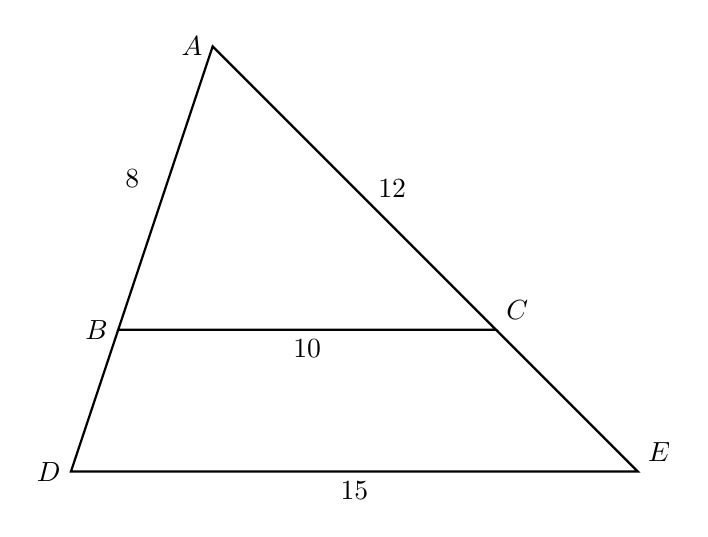
\begin{tikzpicture}[scale=0.6]
         \draw [thick]
         (0,0)node[left]{$B$}--
         (8,0)node[above right]{$C$}--
         (2,6)node[left]{$A$}--cycle;
         \draw [thick]
         (0,0)--
         (-1,-3)node[left]{$D$}--
         (11,-3)node[above right]{$E$}--(8,0);
         \node at (4,0)[below]{$10$};
         \node at (5.3, 3)[right]{$12$};
         \node at (0.3, 2.8)[above]{$8$};
         \node at (5,-3)[below]{$15$};
       \end{tikzpicture}
     \end{flushright}
  
\newpage
\item A dilation with $k=3$ centered at the origin maps $\triangle DEF$ onto $\triangle LMN$. \vspace{0.5cm}
  \begin{multicols}{2}
    The following is given:\\*[0.5cm]
    $DE=10$ \\
    $m\angle E = 40^\circ$ \\
    $m\angle F = 110^\circ$ \\
    $m\angle M = 2x + 10^\circ$ \\
    Fill in the blanks:
    \begin{enumerate}
      \item $D \rightarrow$ \rule{2cm}{0.15mm}
      \item $LM =$ \rule{2cm}{0.15mm}
      \item $m\angle M =$ \rule{2cm}{0.15mm}
      \item Solve for $x$
    \end{enumerate}
  \end{multicols}  \vspace{2cm}

\item Translate $\triangle ABC$ by $(x,y) \rightarrow (x+3, y+4)$. Make a table of the coordinates and plot and label the image on the axes.
  \begin{flushright}
      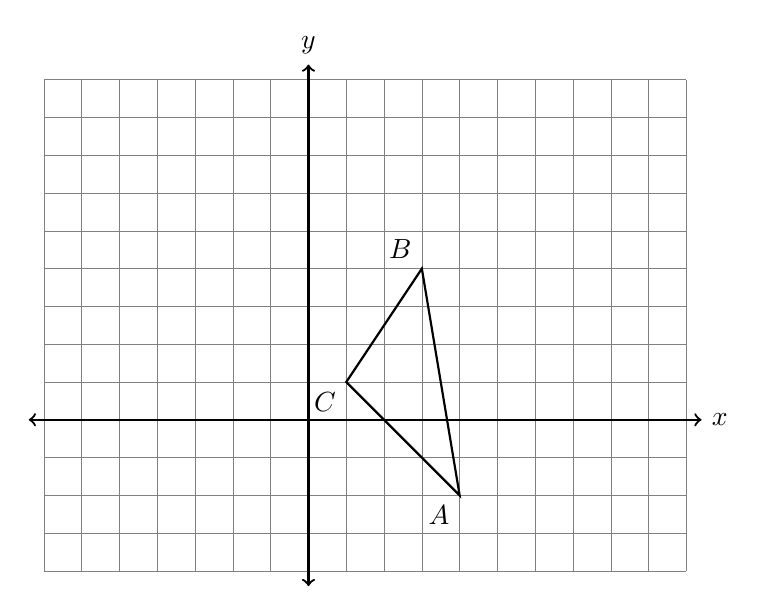
\begin{tikzpicture}[scale=.48]
      \draw [help lines] (-7,-4) grid (10,9);
      \draw [thick, <->] (-7.4,0) -- (10.4,0) node [right] {$x$};
      \draw [thick, <->] (0,-4.4)--(0,9.4) node [above] {$y$};  
      \draw [thick]
        (4,-2) node[below left] {$A$}--
        (3,4) node[above left] {$B$}--
        (1,1) node[below left] {$C$}--cycle;  
    \end{tikzpicture}
  \end{flushright}

\item Given $\triangle JKL \sim \triangle MNO$. $m\angle K = 40^\circ$ and $m\angle M = 100^\circ$.\\
  Find the measure of $\angle N$. \vspace{3cm}

\newpage
\item Apply a translation of $(x,y) \rightarrow (x-4, y-6)$ to $\triangle ABC$. Plot and label the image on the axes below and make a table of its coordinates.
\begin{flushright}
  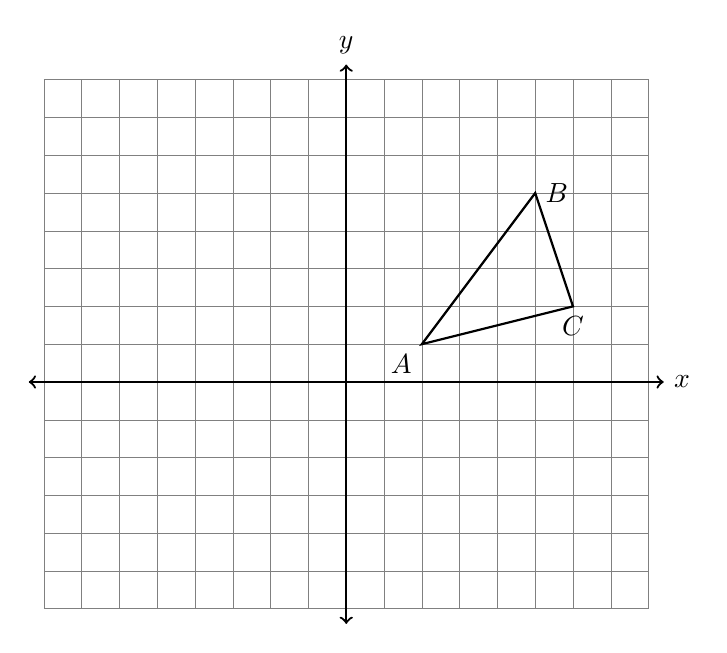
\begin{tikzpicture}[scale=.48]
    \draw [help lines] (-8,-6) grid (8,8);
    \draw [thick, <->] (-8.4,0) -- (8.4,0) node [right] {$x$};
    \draw [thick, <->] (0,-6.4)--(0,8.4) node [above] {$y$};
    \draw [thick]
      (2,1) node[below left] {$A$}--
      (5,5) node[right] {$B$}--
      (6,2) node[below] {$C$}--
      cycle;
  \end{tikzpicture}
\end{flushright}

\item Given isosceles $\triangle ABC$ with $\overline{AC} \cong \overline{AB}$, $m\angle A = x$, $m\angle B = 55$, and $m\angle C=y$. Find $x$ and $y$. \hfill (\emph{the diagram is not to scale})
  \begin{flushright}
  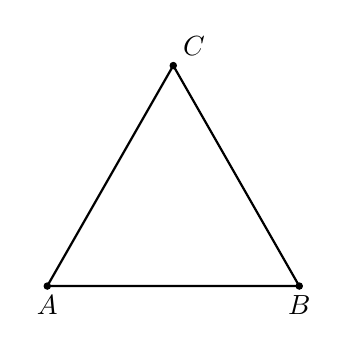
\begin{tikzpicture}[scale=0.8]
    \draw [thick](0,0)--(4,0)--(2,3.5)--(0,0);
    \draw [fill] (0,0) circle [radius=0.05] node[below]{$A$};
    \draw [fill] (4,0) circle [radius=0.05] node[below]{$B$};
    \draw [fill] (2,3.5) circle [radius=0.05] node[above right]{$C$};
  \end{tikzpicture}
  \end{flushright}

\item Given isosceles $\triangle RSU$ with $\overline{UR} \cong \overline{RS}$. If $m\angle UST=140$ find $m\angle U$.
  \begin{flushright}
  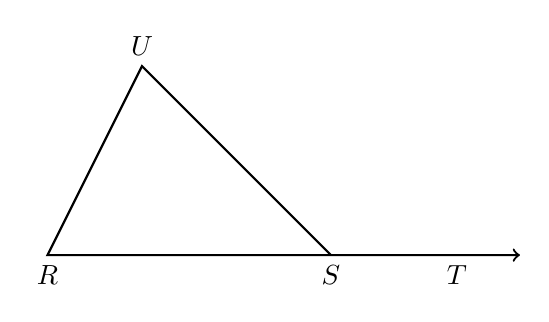
\begin{tikzpicture}[scale=0.8]
    %\draw [->, thick] (0,0)--(5,5);
    \draw [<-, thick] (8,0)--
      (7,0) node[below]{$T$}--
      (0.5,0) node[below]{$R$}--
      (2,3) node[above]{$U$}--
      (5,0) node[below]{$S$};
  \end{tikzpicture}
  \end{flushright} \vspace{3cm}

\newpage
\item Find the area of the parallelogram $ABCD$ shown below, with $AB=9.5$ and height $h=7.1$.
\begin{flushright}
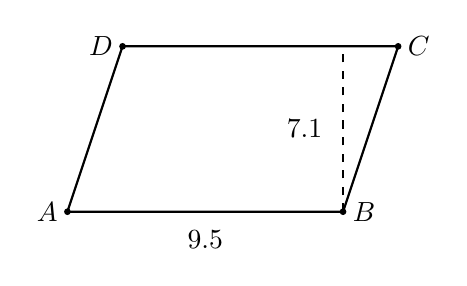
\begin{tikzpicture}[scale=0.7]
  \draw [-, thick] (0,0)--(5,0)--(6,3)--(1,3)--cycle;
  \draw [-, dashed] (5,0)--(5,3);
  \draw [fill] (0,0) circle [radius=0.05] node[left]{$A$};
  \draw [fill] (5,0) circle [radius=0.05] node[right]{$B$};
  \draw [fill] (6,3) circle [radius=0.05] node[right]{$C$};
  \draw [fill] (1,3) circle [radius=0.05] node[left]{$D$};
  \node at (4.3, 1.5){$7.1$};
  \node at (2.5, -0.5){9.5};
\end{tikzpicture}
\end{flushright}

\item Find the sum of the measures of the internal angles of a hexagon. Show the formula.  \vspace{3cm}

\item  A wooden cutting board is $8 \frac{1}{2}$ inches long, 7 inches wide, and $1 \frac{1}{4}$ inches thick. Find the volume of the box. Show the calculation.
\begin{flushright}
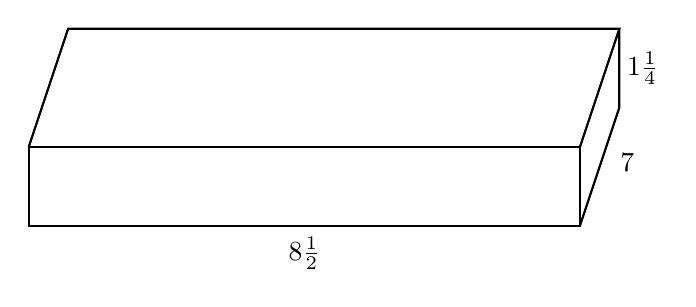
\begin{tikzpicture}[scale=1]
  \draw [-, thick] (0,0)--(7,0)--(7,1)--(0,1)--cycle;
  \draw [-, thick] (0,1)--(0.5,2.5)--(7.5,2.5)--(7,1);
  \draw [-, thick] (7,0)--(7.5,1.5)--(7.5,2.5);
  \node at (7.8, 2){$1 \frac{1}{4}$};
  \node at (3.5, -0.35){$8 \frac{1}{2}$};
  \node at (7.6, 0.8){$7$};
\end{tikzpicture}
\end{flushright} \vspace{3cm}

\item Of two complementary angles, the measure of $\angle A$ is two times that of $\angle B$. Find $m\angle A$. \vspace{3.5cm} 

\newpage
\item An angle bisector is shown below, with $\overrightarrow{AC}$ bisecting $\angle BAD$. Given $m\angle BAC = 6x-5$ and $m\angle BAD = 9x+17$, find $m\angle BAD$. (Show check)
\begin{flushright}
\begin{tikzpicture}[scale=0.7, rotate=30]
\draw [<->, thick] (100:7)node[left]{$B$} 
--(0,0)node[below]{$A$}
--(6,0)node[below]{$D$}--(7,0);
\draw [->, thick] (0,0)--(50:7)node[below right]{$C$};
%\draw [fill] (0,0) circle [radius=0.05] node[below]{$A$};
%\draw [fill] (5,0) circle [radius=0.05] node[below]{$B$};
\end{tikzpicture}
\end{flushright} \vspace{3cm}

\item Angles $APC$ and $CPD$ form a linear pair. $m\angle APC = 10x-10$ and $m\angle CPD = 3x-5$. Find $m\angle CPD$. Check your answer for full credit.
\begin{flushright}
  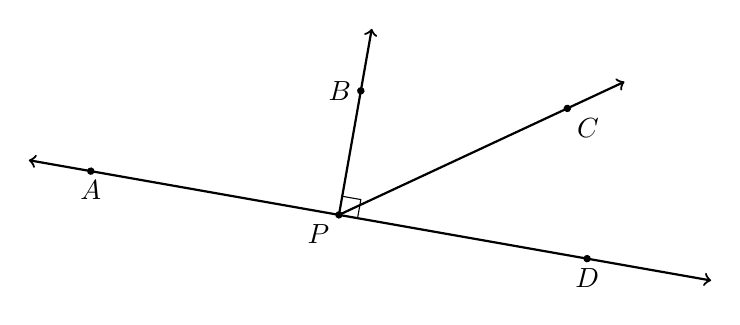
\begin{tikzpicture}[scale=0.8, rotate=-10]
    \draw [->, thick] (0,0)--(35:5);
    \draw [<->, thick] (-5,0)--(6,0);
    \draw [->, thick] (0,0)--(0,3);
    \draw (0,0)++(0.3,0)--++(0,0.3)--+(-0.3,0);
    %\draw [fill] (-1,2.5) circle [radius=0.05] node[left ]{$B$};
    \draw [fill] (35:4) circle [radius=0.05] node[below right]{$C$};
    \draw [fill] (-4,0) circle [radius=0.05] node[below]{$A$};
    \draw [fill] (0,0) circle [radius=0.05] node[below left]{$P$};
    \draw [fill] (0,2) circle [radius=0.05] node[left]{$B$};
    \draw [fill] (4,0) circle [radius=0.05] node[below]{$D$};
  \end{tikzpicture}
  \end{flushright}
  \vspace{5cm}

\newpage
\subsubsection*{Do Not Solve! \\
Model the situation with an equation in terms of $x$.}

\item Given $\overline{ABC}$, with $AB=2x-1$, $BC=3x+7$, and $AC=21$. Find $x$. \vspace{1cm}
  \begin{flushright}
    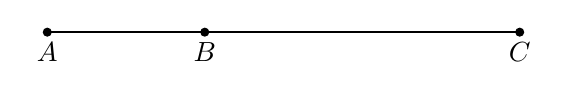
\begin{tikzpicture}
      \draw [-, thick] (0,0) node[below]{$A$}--
      (2,0) node[below]{$B$}--
      (6,0) node[below]{$C$};
      \draw [fill] (0,0) circle [radius=0.05];
      \draw [fill] (2,0) circle [radius=0.05];
      \draw [fill] (6,0) circle [radius=0.05];
    \end{tikzpicture}
    \end{flushright} \vspace{1cm}
  
\item Given $m\angle 3 = x+35$ and $m\angle 5 = 4x-25$. Find $x$. 
  \begin{flushright}
  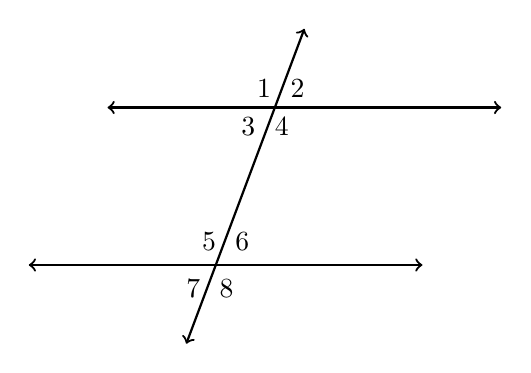
\begin{tikzpicture}
    \draw [<->, thick] (3,2)--(8,2);
    \draw [<->, thick] (2,0)--(7,0);
    \draw [<->, thick] (4,-1)--(5.5,3);
    \node at (4.5,0.3) [left]{$5$};
    \node at (4.5,0.3) [right]{$6$};
    \node at (4.3,-0.3) [left]{$7$};
    \node at (4.3,-0.3) [right]{$8$};
    \node at (5.2,2) [above left]{$1$};
    \node at (5.2,2) [above right]{$2$};
    \node at (5,2) [below left]{$3$};
    \node at (5,2) [below right]{$4$};
  \end{tikzpicture}
  \end{flushright} \vspace{0.5cm}

\item In the diagram below $m\angle AOB = 6x+5$ and $m\angle COB = 8x+15$. Find $x$. %\vspace{0.25cm}
  \begin{flushright}
  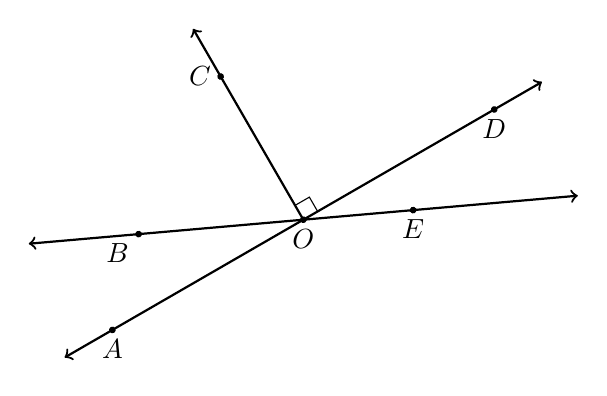
\begin{tikzpicture}[scale=0.7, rotate=30]
  \draw [<->, thick] (-25:5)--(0,0)--(155:5);
  \draw [<->, thick] (-5,0)--(5,0);
  \draw [->, thick] (0,0)--(0,4);
  \draw (0,0)++(0.3,0)--++(0,0.3)--+(-0.3,0);
  %\draw [fill] (-1,2.5) circle [radius=0.05] node[left ]{$B$};
  \draw [fill] (155:3) circle [radius=0.05] node[below left]{$B$};
  \draw [fill] (-4,0) circle [radius=0.05] node[below]{$A$}; 
  \draw [fill] (0,0) circle [radius=0.05] node[below]{$O$};
  \draw [fill] (0,3) circle [radius=0.05] node[left]{$C$};
  \draw [fill] (4,0) circle [radius=0.05] node[below]{$D$};
  \draw [fill] (-25:2) circle [radius=0.05] node[below]{$E$};
  \end{tikzpicture}
  \end{flushright}

\item The point $K$ is the midpoint of $\overline{JL}$, $JK=3x+15$, and $JL=9x+9$. Find $x$.  \vspace{1cm}
  \begin{flushright}
    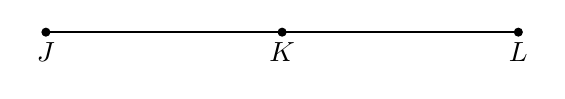
\begin{tikzpicture}
      \draw [-, thick] (0,0) node[below]{$J$}--
      (3,0) node[below]{$K$}--
      (6,0) node[below]{$L$};
      \draw [fill] (0,0) circle [radius=0.05];
      \draw [fill] (3,0) circle [radius=0.05];
      \draw [fill] (6,0) circle [radius=0.05];
    \end{tikzpicture}
    \end{flushright} \vspace{2cm}

\end{enumerate}
\end{document}